% Chương "Kết quả thực hiện" - BTL Đại số tuyến tính: Chuẩn của ma trận
% Biên dịch được bằng pdfLaTeX hoặc XeLaTeX. Hình lấy từ thư mục ../ket_qua (bản Python, thông số mặc định).
% Khi ghép vào báo cáo chính: bỏ phần mở đầu, dòng \setcounter{section} và cặp \begin{document}...\end{document},
% rồi đổi lại \section/\subsection/\subsubsection cho khớp cấp đề mục của báo cáo.
\documentclass[12pt,a4paper]{article}

\usepackage{iftex}
\ifPDFTeX
  \usepackage[utf8]{inputenc}
  \usepackage[T5]{fontenc}
\else
  \usepackage{fontspec}
\fi
\usepackage[vietnamese]{babel}
\usepackage[margin=2.5cm]{geometry}
\usepackage{amsmath,amssymb}
\usepackage{booktabs}
\usepackage{adjustbox}
\usepackage{graphicx}
\usepackage{float}
\usepackage[hidelinks]{hyperref}

\graphicspath{{../ket_qua/}}

% Ký hiệu dùng chung
\newcommand{\chuan}[1]{\left\lVert #1 \right\rVert}
\newcommand{\doC}{\,^{\circ}\mathrm{C}}

\begin{document}

\setcounter{section}{3} % để chương này được đánh số 4

\section{Kết quả thực hiện}

% ======================================================================================
\subsection{Kết quả tính toán các chuẩn trên ma trận cụ thể}

Bài toán ứng dụng được khảo sát là một tấm tản nhiệt CPU bằng nhôm kích thước $10\times 10$~cm, độ dày 1~mm.
Tấm nhôm được mô hình hóa bằng cách chia lưới $20\times 20$ điểm, dẫn đến việc thiết lập một hệ phương trình
tuyến tính có ma trận hệ số $A$ với kích thước $400\times 400$.

Trước khi tính toán trên hệ phương trình thực tế, các hàm tính chuẩn tự cài đặt đã được kiểm thử trên các ma trận
ví dụ cỡ nhỏ. Kết quả đối chiếu ở Bảng~\ref{tab:kiemthu} cho thấy các hàm tự cài đặt cho kết quả khớp với lý thuyết.

\begin{table}[H]
\centering
\caption{Kết quả kiểm thử các chuẩn ma trận trên ví dụ cơ bản}
\label{tab:kiemthu}
\begin{tabular}{cccc}
\toprule
Ký hiệu & Ma trận & Giá trị chuẩn tính được & Đánh giá \\
\midrule
$M_1$ & $\begin{bmatrix} 2 & 5 & 4\\ 6 & 4 & 3\\ 5 & 3 & 5 \end{bmatrix}$ & $\chuan{M_1}_1 = 13$ & Khớp lý thuyết \\[16pt]
$M_2$ & $\begin{bmatrix} -3 & 5 & -2\\ 1 & -7 & 4\\ 2 & 0 & 9 \end{bmatrix}$ & $\chuan{M_2}_\infty = 12$ & Khớp lý thuyết \\[16pt]
$M_3$ & $\begin{bmatrix} 5 & 2\\ 2 & 5 \end{bmatrix}$ & $\chuan{M_3}_2 = 7$ & Khớp lý thuyết \\[12pt]
$M_4$ & $\begin{bmatrix} 1 & 3\\ 0 & 2 \end{bmatrix}$ & $\chuan{M_4}_2 = 3.702$ & Khớp lý thuyết \\
\bottomrule
\end{tabular}
\end{table}

Tiếp theo, tiến hành tính các chuẩn của ma trận hệ số $A$ ($400\times 400$) của mô hình tản nhiệt.
Với $h = 100$~W/m\textsuperscript{2}K, $k = 200$~W/mK, $t = 1$~mm, $T_{\mathrm{CPU}} = 80\doC$, $T_{\text{phòng}} = 25\doC$,
ta có $m^2 = 2h/(kt) = 1000~\mathrm{m}^{-2}$. Bước lưới $dx = L/21$, suy ra hằng số lưới $c = m^2\, dx^2 \approx 0.02268$.
Bảng~\ref{tab:chuanA} tổng hợp kết quả tính chuẩn của $A$.

\begin{table}[H]
\centering
\caption{Các chuẩn của ma trận hệ số $A$ ($400\times 400$)}
\label{tab:chuanA}
\begin{adjustbox}{max width=\textwidth}
\begin{tabular}{lccc}
\toprule
Loại chuẩn & Tự cài đặt & Hàm thư viện & Công thức giải tích \\
\midrule
Chuẩn cột ($\chuan{A}_1$) & 8.022676 & 8.022676 & $8 + c$ \\
Chuẩn hàng ($\chuan{A}_\infty$) & 8.022676 & 8.022676 & $8 + c$ \\
Chuẩn Frobenius ($\chuan{A}_F$) & 89.402282 & 89.402282 & $\sqrt{N^2(4+c)^2 + 4N(N-1)}$ \\
Chuẩn phổ ($\chuan{A}_2$) & 7.977999 & 7.977999 & $\lambda_{\max}$ \\
\bottomrule
\end{tabular}
\end{adjustbox}
\end{table}

Kết quả cho thấy phương pháp lặp lũy thừa để tìm chuẩn 2 hội tụ sát với trị riêng lớn nhất $\lambda_{\max}$ sau 638 vòng lặp.
Đồng thời, kết quả tính toán số học cũng thỏa mãn các bất đẳng thức về chuẩn ma trận, với $r = \operatorname{rank}(A) = 400$:
\begin{align*}
\chuan{A}_2 \le \chuan{A}_F \le \sqrt{r}\,\chuan{A}_2 &\implies 7.9780 \le 89.4023 \le 159.5600,\\
\chuan{A}_2 \le \sqrt{\chuan{A}_1 \cdot \chuan{A}_\infty} &\implies 7.9780 \le 8.0227.
\end{align*}

% ======================================================================================
\subsection{Kết quả chạy chương trình đánh giá sai số hệ phương trình}

\subsubsection{Độ ổn định của hệ phương trình và sai số cảm biến}

Số điều kiện (condition number) của ma trận $A$ được xác định thông qua chuẩn ma trận: $\kappa_1 = \kappa_\infty = 165.18$
và $\kappa_2 = \lambda_{\max}/\lambda_{\min} = 118.45$. Theo quy tắc kinh nghiệm, giá trị $\kappa \approx 118$ cho thấy
hệ phương trình thuộc dạng ổn định, việc tính toán chỉ mất khoảng 2 chữ số chính xác.

Để đánh giá mức độ lan truyền sai số, nhóm giả định các cảm biến đo nhiệt độ tại cạnh CPU có nhiễu ngẫu nhiên
$\pm 0.5\doC$ (sai số vế phải $b$). Bảng~\ref{tab:camBien} cho thấy mức độ khuếch đại sai số luôn nằm trong cận lý thuyết
\[
\frac{1}{\kappa}\,\frac{\chuan{\delta b}}{\chuan{b}} \le \frac{\chuan{\delta\theta}}{\chuan{\theta}} \le \kappa\,\frac{\chuan{\delta b}}{\chuan{b}}.
\]

\begin{table}[H]
\centering
\caption{Sai số tương đối của nghiệm khi cảm biến sai $\pm 0.5\doC$}
\label{tab:camBien}
\begin{adjustbox}{max width=\textwidth}
\begin{tabular}{lcccc}
\toprule
Chuẩn & $\chuan{\delta b}/\chuan{b}$ & $\chuan{\delta\theta}/\chuan{\theta}$ & Cận dưới & Cận trên \\
\midrule
Chuẩn 1 & $4.060\times 10^{-3}$ & $1.749\times 10^{-3}$ & $2.458\times 10^{-5}$ & $0.6706$ \\
Chuẩn 2 & $4.661\times 10^{-3}$ & $2.232\times 10^{-3}$ & $3.935\times 10^{-5}$ & $0.5521$ \\
Chuẩn $\infty$ & $8.490\times 10^{-3}$ & $5.075\times 10^{-3}$ & $5.140\times 10^{-5}$ & $1.402$ \\
\bottomrule
\end{tabular}
\end{adjustbox}
\end{table}

Thực tế, khi cảm biến sai $\pm 0.5\doC$, sai lệch nhiệt độ lớn nhất trên toàn bộ bề mặt tấm tản nhiệt chỉ là $0.24\doC$
(nhỏ hơn rất nhiều so với cận trên dự báo là $9.6\doC$ dựa trên chuẩn vô cùng). Khi chọn $b$ theo hướng $u_1$ và nhiễu
theo hướng $u_n$ của SVD, hệ số khuếch đại đạt đúng $\kappa_2 = 118.45$, nên cận trên là chặt.
Điều này cho thấy kết quả đủ tin cậy với sai số cảm biến $\pm 0.5\doC$.

\subsubsection{Sự đánh đổi khi chia lưới mịn}

Việc chia lưới mô phỏng nhỏ hơn sẽ làm kết quả tính toán tiệm cận hơn với trường nhiệt chính xác, tuy nhiên đồng thời
cũng làm tăng độ nhạy cảm của hệ thống đối với sai số đầu vào.

\begin{table}[H]
\centering
\caption{Ảnh hưởng của độ mịn lưới đến số điều kiện $\kappa_2$ và sai số mô hình}
\label{tab:luoi}
\begin{adjustbox}{max width=\textwidth}
\begin{tabular}{cccccc}
\toprule
Kích thước ($N$) & Số ẩn & $\kappa_2$ (tự tính) & $\kappa_2$ (lý thuyết) & $q$ (Jacobi) & Sai số mô hình \\
\midrule
$5\times 5$   & 25   & 9.51   & 9.51   & 0.93506 & 1.52\% \\
$10\times 10$ & 100  & 32.37  & 32.37  & 0.97976 & 0.71\% \\
$20\times 20$ & 400  & 118.45 & 118.45 & 0.99436 & 0.35\% \\
$40\times 40$ & 1600 & 452.02 & 452.02 & 0.99851 & 0.17\% \\
\bottomrule
\end{tabular}
\end{adjustbox}
\end{table}

\begin{figure}[H]
\centering
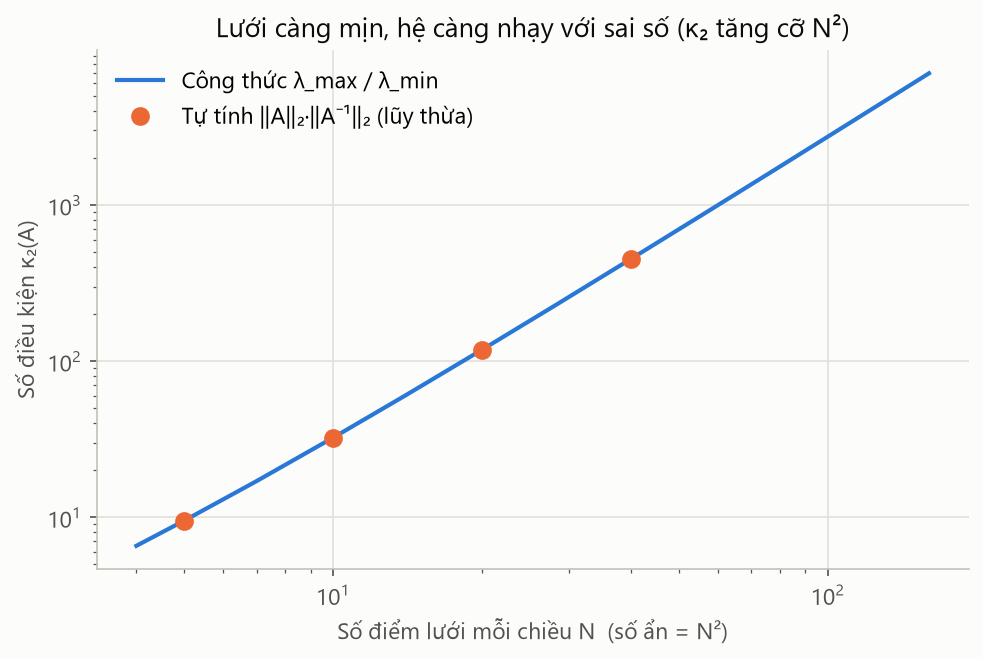
\includegraphics[width=0.75\textwidth]{hinh2_so_dieu_kien.png}
\caption{Số điều kiện tăng xấp xỉ theo $N^2$ khi chia lưới mịn hơn}
\label{fig:dieuKien}
\end{figure}

Như thể hiện ở Bảng~\ref{tab:luoi} và Hình~\ref{fig:dieuKien}, khi số điểm lưới mỗi chiều tăng gấp đôi, sai số mô hình giảm đi
khoảng một nửa nhưng số điều kiện $\kappa_2$ tăng gần 4 lần (từ 3.4 đến 3.8 lần). Tuy vậy, ngay cả ở lưới 400 ẩn, hệ vẫn ổn định
so với các ma trận kém điều kiện (ví dụ: ma trận Hilbert cấp 10 đã có $\kappa_2 \approx 1.6\times 10^{13}$).

\subsubsection{Thuật toán dừng trong giải lặp}

Hệ phương trình $400\times 400$ được giải bằng các phương pháp lặp. Chuẩn vô cùng đóng vai trò then chốt trong việc xác định hệ số co.
Với Jacobi, $q = \chuan{B}_\infty = 0.99436$. Với Gauss-Seidel, $q = \max_i r_i/(1-p_i) = 0.98879$, trong đó $p_i$ và $r_i$ là tổng
$|b_{ij}|$ bên trái và bên phải đường chéo ở hàng $i$. Do $A$ trội đường chéo chặt nên $q < 1$, đảm bảo phương pháp lặp luôn hội tụ.
Với yêu cầu sai số $\varepsilon = 10^{-3}\doC$, ta tiến hành đánh giá điều kiện dừng.

Nếu áp dụng tiêu chí dừng ngây thơ (chỉ dựa vào $\chuan{x^{(k)} - x^{(k-1)}} \le \varepsilon$), thuật toán Gauss-Seidel sẽ dừng sớm ở
vòng 181, gây ra sai số thực tế là $0.028\doC$ (gấp 28 lần mức cho phép). Ngược lại, khi sử dụng đánh giá hậu nghiệm dựa trên chuẩn ma trận
\[
\frac{q}{1-q}\chuan{x^{(k)} - x^{(k-1)}}_\infty \le \varepsilon,
\]
thuật toán dừng ở vòng 313, với sai số thật là $3.3\times 10^{-4}\doC$, đạt yêu cầu. Bảng~\ref{tab:lap} so sánh hai phương pháp.

\begin{table}[H]
\centering
\caption{So sánh Jacobi và Gauss-Seidel với $\varepsilon = 10^{-3}\doC$}
\label{tab:lap}
\begin{adjustbox}{max width=\textwidth}
\begin{tabular}{lcccccc}
\toprule
 & & Tiên nghiệm & \multicolumn{2}{c}{Dừng hậu nghiệm} & \multicolumn{2}{c}{Dừng ngây thơ} \\
\cmidrule(lr){4-5}\cmidrule(lr){6-7}
Phương pháp & $q$ & dự báo (vòng) & Số vòng & Sai số thật ($^{\circ}$C) & Số vòng & Sai số thật ($^{\circ}$C) \\
\midrule
Jacobi       & 0.99436 & 2601 & 634 & $3.29\times 10^{-4}$ & 327 & $5.86\times 10^{-2}$ ($59\varepsilon$) \\
Gauss-Seidel & 0.98879 & 1269 & 313 & $3.30\times 10^{-4}$ & 181 & $2.84\times 10^{-2}$ ($28\varepsilon$) \\
\bottomrule
\end{tabular}
\end{adjustbox}
\end{table}

\begin{figure}[H]
\centering
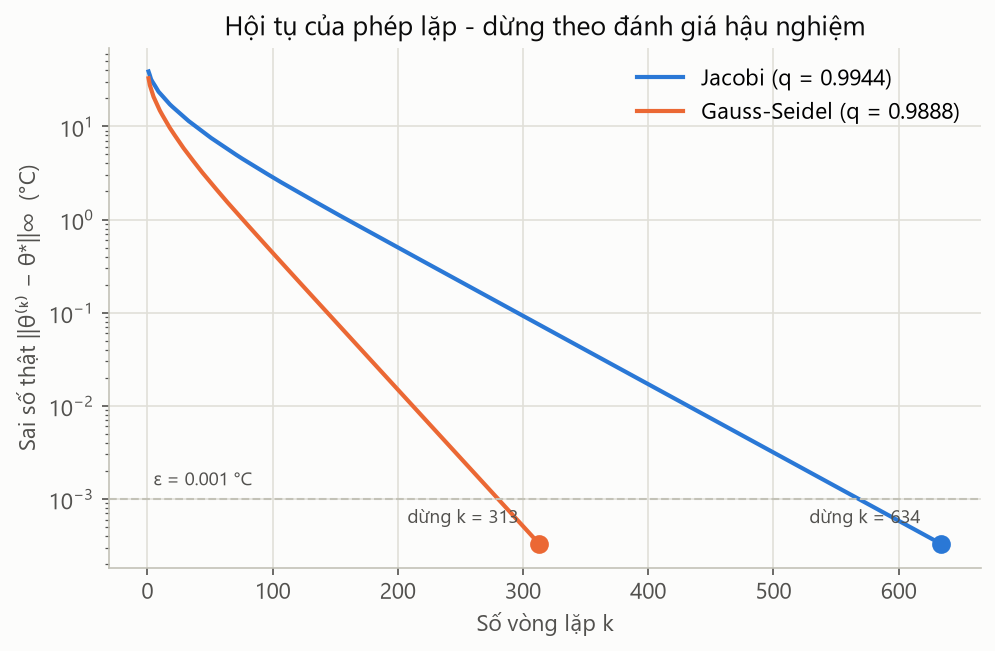
\includegraphics[width=0.75\textwidth]{hinh3_hoi_tu.png}
\caption{Sự hội tụ của phép lặp và vai trò của điều kiện dừng hậu nghiệm}
\label{fig:hoiTu}
\end{figure}

\begin{figure}[H]
\centering
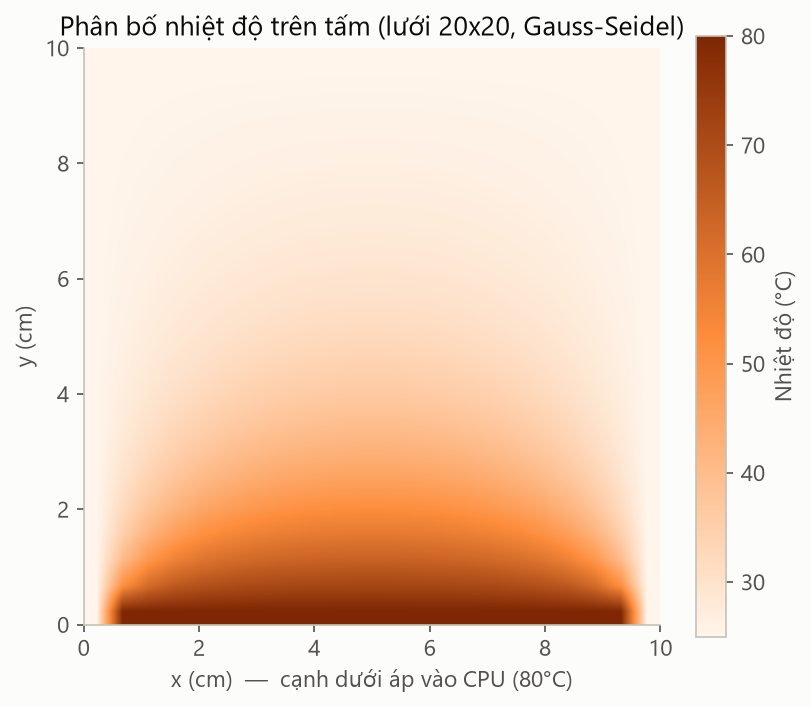
\includegraphics[width=0.6\textwidth]{hinh1_ban_do_nhiet.png}
\caption{Bản đồ phân bố nhiệt độ trên tấm tản nhiệt CPU (kết quả Gauss-Seidel)}
\label{fig:banDoNhiet}
\end{figure}

Kết quả tại Hình~\ref{fig:banDoNhiet} cho thấy nhiệt độ phân bố hợp lý: điểm lưới nóng nhất, sát CPU, đạt $71.4\doC$
(bản thân cạnh CPU là $80\doC$) và nhiệt độ giảm dần, còn $31.6\doC$ tại khu vực tâm tấm tản nhiệt.

% ======================================================================================
\subsection{Kết quả ứng dụng đo độ chênh lệch dữ liệu / ảnh}

Chuẩn ma trận tiếp tục được ứng dụng để đánh giá độ chính xác so với dữ liệu camera nhiệt mô phỏng. Ảnh camera bản chất là một ma trận $C$
kích thước $128\times 128$. Do nhiễu tín hiệu (nhiễu Gauss, độ lệch chuẩn $2\doC$), ảnh camera xuất hiện nhiều hạt và lệch so với trường nhiệt chuẩn.
Khoảng cách chênh lệch này được đo bằng chuẩn Frobenius:
\[
\frac{\chuan{C - \theta}_F}{\chuan{\theta}_F} = 11.85\%.
\]

Nhóm tiến hành phân tích giá trị kỳ dị (SVD) để tách lớp bức ảnh, loại bỏ nhiễu. Theo định lý Eckart--Young, độ lệch của ảnh nén $C_k$ so với ảnh gốc $C$
được xác định chính xác bởi các giá trị kỳ dị:
\[
\chuan{C - C_k}_F = \sqrt{\sigma_{k+1}^2 + \dots + \sigma_n^2}, \qquad \chuan{C - C_k}_2 = \sigma_{k+1}.
\]
Bảng~\ref{tab:eckart} kiểm chứng hai đẳng thức này bằng số.

\begin{table}[H]
\centering
\caption{Kiểm chứng định lý Eckart--Young trên ảnh camera}
\label{tab:eckart}
\begin{tabular}{ccccc}
\toprule
$k$ & $\chuan{C - C_k}_F$ & $\sqrt{\sum_{i>k}\sigma_i^2}$ & $\chuan{C - C_k}_2$ & $\sigma_{k+1}$ \\
\midrule
1  & 352.19 & 352.19 & 237.97 & 237.97 \\
2  & 259.64 & 259.64 & 64.81  & 64.81 \\
3  & 251.42 & 251.42 & 44.16  & 44.16 \\
10 & 226.13 & 226.13 & 38.91  & 38.91 \\
50 & 113.97 & 113.97 & 22.71  & 22.71 \\
\bottomrule
\end{tabular}
\end{table}

\begin{table}[H]
\centering
\caption{Hiệu quả giảm nhiễu và nén dữ liệu khi giữ lại $k$ thành phần SVD}
\label{tab:svd}
\begin{tabular}{cccc}
\toprule
Số thành phần ($k$) & Lệch ảnh camera & Lệch trường thật & Dung lượng lưu trữ \\
\midrule
1  & 16.15\% & 11.33\% & 1.6\% \\
2  & 11.90\% & 3.44\%  & 3.1\% \\
3  & 11.53\% & 2.77\%  & 4.7\% \\
10 & 10.37\% & 5.72\%  & 15.7\% \\
50 & 5.23\%  & 10.63\% & 78.4\% \\
\bottomrule
\end{tabular}
\end{table}

\begin{figure}[H]
\centering
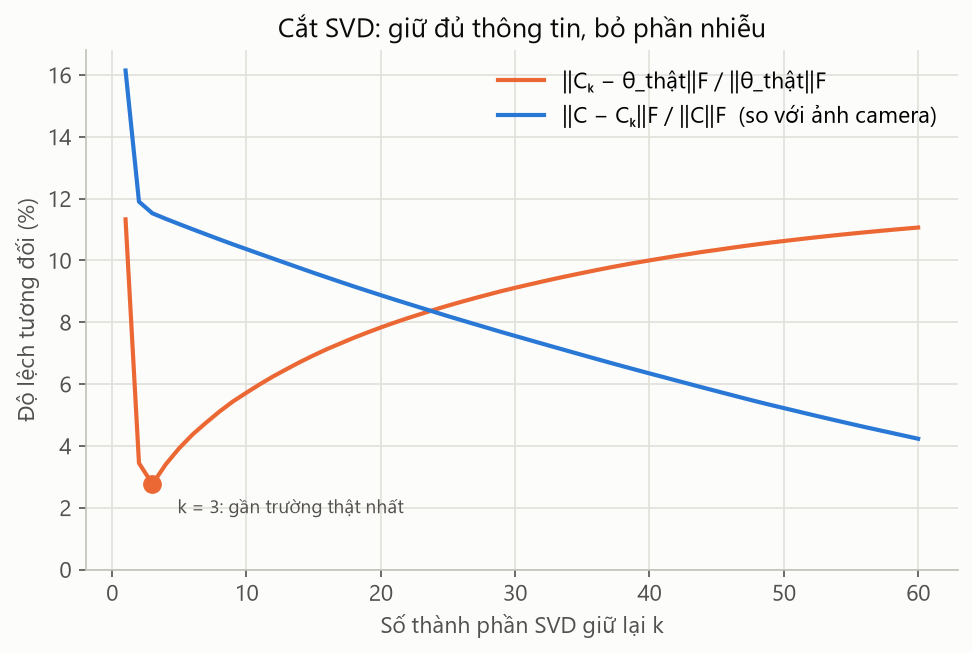
\includegraphics[width=0.75\textwidth]{hinh5_do_lech_svd.png}
\caption{Độ lệch dữ liệu tương đối phụ thuộc vào số lượng thành phần SVD ($k$)}
\label{fig:doLech}
\end{figure}

Phân tích từ Bảng~\ref{tab:svd} và Hình~\ref{fig:doLech} chỉ ra một kết quả đáng chú ý: do trường nhiệt rất trơn, ma trận phân bố nhiệt
xấp xỉ rất tốt bằng ma trận hạng thấp. Trong khi đó, nhiễu lại phân tán đều trên mọi thành phần phổ.

\begin{figure}[H]
\centering
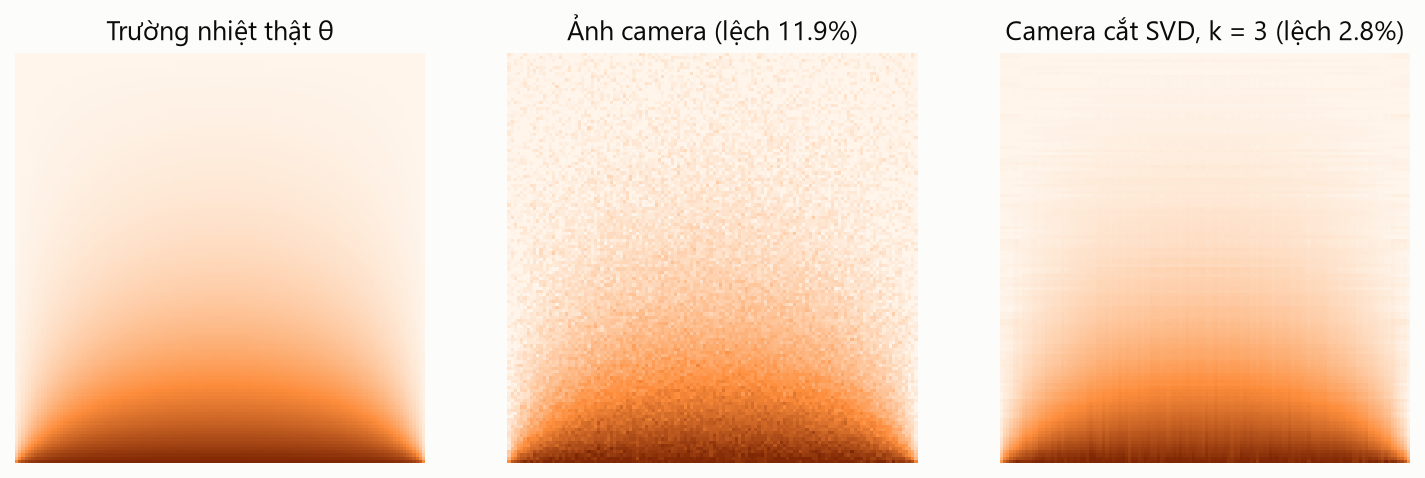
\includegraphics[width=\textwidth]{hinh4_anh_camera.png}
\caption{So sánh hình ảnh trường nhiệt trước và sau khi làm sạch bằng SVD}
\label{fig:anhCamera}
\end{figure}

Như minh họa tại Hình~\ref{fig:anhCamera}, chỉ cần giữ lại $k = 3$ thành phần, phương pháp đã loại bỏ phần lớn nhiễu, giảm độ lệch so với trường nhiệt thật
từ 11.85\% xuống 2.77\%, mức thấp nhất trong các giá trị $k = 1,\dots,60$ đã khảo sát. Việc giữ thêm thành phần ($k > 3$) không làm ảnh tốt hơn
mà ngược lại sẽ kéo theo cả nhiễu. Hơn nữa, ma trận ảnh đã được nén, chỉ còn chiếm 4.7\% dung lượng lưu trữ so với bức ảnh gốc ban đầu.

Số liệu trong chương này lấy từ chương trình Python với seed ngẫu nhiên cố định 2026.

\end{document}
